%\documentclass[]{iopart}
%
%\usepackage{graphicx}% Include figure files
%\usepackage{dcolumn}% Align table columns on decimal point1
%\usepackage{bm}% bold math
%\usepackage[caption=false]{subfig}
%
%\begin{document}
%\title{Experimental setup}

\chapter[Experimental setup]{Experimental setup\label{ch:setup}}

\begin{abstract}
The experimental setup is described in details in the PhD theses of Reijnders \cite{Reijnders2010} and Taban \cite{Taban2009}. In this chapter, only the essential parts of the setup (important details and changes) are given.
The beam line and the MOT chamber are described in the first two sections. The laser setup is shown in section \ref{sec:lasers}. Information about the calibration and the resolution of the detector assembly (which is also simply named detector), playing an important role in the measurement of chapters \ref{ch:tempmea} and \ref{ch:currentmea}, are given in section \ref{sec:calibrationMCP} and section \ref{sec:resoMCP}.
\end{abstract}

\clearpage

\section{Beam line}
The experimental setup is schematically drawn in figure \ref{fig:beamline}.
\begin{figure}[tbh!]
	\centering
		\includegraphics[width=1\linewidth]{pics/setup/beamline}
	\caption{Schematic drawing of the beam line used to measure the properties of the UCIS. The negative $x$-direction is pointing toward the reader. \label{fig:beamline}}
\end{figure}
The ions are created in the magneto-optical trap (MOT) chamber on the left hand side of the figure at $z=0$ and travel about 1.5~m in the beam line until the detector, shown on the right hand side. The MOT is located in a vacuum chamber, where the typical pressure is kept below $10^{-8}$~mbar by a pumping system consisting of two ion getter pumps, not shown in figure \ref{fig:beamline}. The MOT chamber is discussed in section \ref{MOTchamber}. The first valve is used to keep the pressure in the MOT chamber independent from the one in beam line, if needed. A pair of deflector plates are used to steer the beam in the $x$ and $y$-directions. A bellows, right after the deflectors, permits to rotate the beam line including the detector within an angle of about $5\,^{\circ}$. A retractable Faraday cup can be inserted in the beam line and with the use of an electrometer, the charge of ion bunches and eventually the current of an ion beam can be measured. The detector assembly is made up of a multichannel plate (MCP) detector, a phosphor screen and a CCD camera. The required calibration is discussed in section \ref{sec:calibrationMCP}. The MCP is kept at a low pressure with an ion getter pump, when the second valve is closed. The same ion pump is used to keep the pressure in the beam line at about $10^{-7}$~mbar, when the second valve is open. The turbo pump, connected with the beam line through the third valve, is used to pre-pump the beam line. During the experiment, the third valve is kept closed and the turbo pump is not running. 


\section{Magneto-optical trap chamber} \label{MOTchamber}
The UCIS setup uses a standard $^{85}$Rb magneto-optical trap configuration \cite{Metcalf_Book_99}. Atoms are cooled with three orthogonal pairs of counter propagating circularly polarized laser beams (trapping lasers) and are trapped by a quadrupole magnetic field. The magnetic field gradient of about 1~G/mm is generated by two coils placed in an anti-Helmholtz configuration. The trapping beams together with the magnetic field gradient slow down and trap the atoms in the center of the MOT, where the origin of the coordinate system is located. The MOT contains about $2 \times 10^8$ $^{85}$Rb atoms within a \textit{rms}-radius of about 1~mm. 

The relevant hyperfine energy levels of $^{85}$Rb are plotted in figure \ref{fig:RbLevels}, where the used laser transitions are also presented. Details about the laser setup are given in section \ref{sec:lasers}.
\begin{figure}[tbh!]
	\centering
	\includegraphics[width=0.5\textwidth]{pics/setup/leveldiagram}
	\caption{The relevant hyperfine energy levels of $^{85}$Rb and the used laser transitions (see next section). The continuum marked by $\infty$ is the ionized state. The figure is edited from reference \cite{Claessens06}. \label{fig:RbLevels}}
\end{figure}
The atoms that are trapped in the MOT, are continuously excited by the trapping laser to the 5P$_{3/2}$-F=4 state, and then decay back to the 5S$_{1/2}$-F=3 ground state. However, since the hyperfine levels are not that far apart, some of the trapping laser power will actually excite the transition to the 5P$_{3/2}$-F=3 state. These atoms can than decay to the ``wrong'' ground state 5S$_{1/2}$-F=2. In order to make sure that these atoms do not get pumped to that state, a repump laser is needed. This pumps the atoms back to the 5P$_{3/2}$-F=3 state, from where they can also decay to the ``right'' ground state, 5S$_{1/2}$-F=3. The repump laser is left on all time and its power is about 10 times less than the power of the trapping laser.

A schematic representation of the vacuum chamber can be found in figure \ref{fig:setup_MOT}.
\begin{figure}[tbh!]
	\centering
		\includegraphics[width=0.7\linewidth]{pics/setup/setup_MOT}
	\caption{Schematic overview of the vacuum chamber that contains the MOT and accelerator structure \cite{Taban2009}. One of the trapping laser beam pairs is shown, namely the horizontal beam pair. This pair consists of two separate laser beams, which are reflected by mirrors before they reach the MOT. It is not exactly horizontal, because in that case the mirror on the right would block the outcoming ion beam. The other pairs are diagonal beams in the $(x,y)$-plane, which are back-reflected. The coils that create the magnetic field gradient are also indicated in the figure. Finally, there are two cameras observing the fluorescence of the MOT, only the top one is shown. The side camera is behind the setup, looking toward the reader. \label{fig:setup_MOT}}
\end{figure}
The electric field strength at the starting point $z=0$ is 0.37 kV/cm per kV input voltage $V_a$ and the energy gained by an ion is $U = e V_a/2.05$, where $e$ is the elementary charge. An ion gains about half of energy applied to the electrodes since the MOT is located half way in between the two electrodes \cite{Taban2009}. The accelerator is rotationally symmetric and designed for acceleration voltages up to 30~kV. With a DC accelerating field, the exit of the accelerator forms an aperture lens with a negative focal length $f_0=33$~mm (``exit kick'' effect), which is independent of the acceleration voltage. For more details of the accelerator structure see \cite{Taban2009}. 

As the trapping lasers continuously excite the trapped atoms, they send out spontaneously emitted photons. Two CCD cameras observe the fluorescence of the MOT, one from the top and one from the side, continuously determining the density and the dimension of the MOT. The number of trapped atoms $N$ is given by
\begin{equation}
	N = K \frac{P \lambda}{h c \Gamma f },
\end{equation}
where $P$ is the power of the emitted light, $\lambda=780$~nm is the wavelength of the emitted light, $h$ is Planck's constant, $\Gamma = 2 \pi \cdot 5.98$~MHz is the decay rate from the excited state, $c$ is the speed of light, $f \approx 0.5$ is the fraction of excited atoms and finally $K$ is a calibration constant. Details on the geometrical configuration and the calibration of the cameras can be found in \cite{Hermans10}. 


\section{Laser setup} \label{sec:lasers}
Lasers form an important part of the setup. They are needed to cool down and trap the atoms, and also to ionize the cooled atoms. Four different lasers are used in the lab and their properties are summarized in table \ref{tab:lasers}.
\begin{table}[tbh!]
\caption{\label{tab:lasers} Lasers used in the experiments.}
\begin{center}
  \begin{tabular}{ | l | l | l | l | l | }
  \hline
  Laser 				& Used to           & Wavelength & Power / Energy  	& Pulse length					\\ \hline
  Toptica DLX 110 		& trap		& 780 nm 		& 900~mW		& CW		 					\\
  Toptica DL 100 		& repump 		& 780 nm 		& 100~mW 		& CW		  					\\
  Quanta-Ray PDL3 		& ionize		& 479.1 nm 		& 0.1~mJ			& 2.5~ns \textit{rms}	\\
  Toptica TA-SHG 110 	& ionize		& 479.1 nm 		& 250~mW 		& CW							\\ \hline
  \end{tabular}
\end{center}
\end{table}

The trapping and repump laser need to be stabilized to within a few megahertz. For the trapping laser beam, this is achieved with modulation transfer spectroscopy. The repump laser is locked with respect to the trapping laser, separated 3~GHz in frequency. More details about the laser locking can be found in \cite{Reijnders2010}. 
The difference in frequency between the trapping laser and excitation laser is very small ($\Delta f=-14.5$~MHz), therefore a single laser is used for both transitions. Moreover, the laser power needed for the excitation laser beam is only a small fraction of that needed for the trapping laser beams since the trapping laser beams are much larger than the excitation laser beam. The power of the trapping laser beams is 250~mW in total, while the excitation laser beam uses at most 10~mW of it. The detuning and intensity of the excitation and trapping laser beams are controlled using acousto-optic modulators (AOMs) which in turn are computer controlled by a programmable pattern generator (PPG). The PPG has an internal clock that operates at 50~MHz, so its time resolution is 20~ns. The PPG is used to synchronize and computer control most of the experimental setup.

The ionization transition is that of the excited atoms from any of the 5P$_{3/2}$ states to just above the ionization threshold. Note that atoms can only be ionized if they are first excited. For the experiment presented in this thesis (chapters \ref{ch:tempmea} and \ref{ch:currentmea}), the CW ionization laser is used. The pulsed dye laser is used as an ionization laser only during the calibration of the detector, see section \ref{sec:calibrationMCP}. The continuous ionization laser beam can be switched on and off with an acousto-optical deflector (AOD), which is also computer controlled.

The photo-ionization takes place in the small region of the atom cloud where both the excitation laser and ionization laser are present, the core region. This is schematically represented in figure \ref{fig:coreVolume}.
\begin{figure}[tbh!]
	\centering
		\includegraphics[width=0.4\linewidth]{pics/setup/coreVolume}
	\caption{Schematic representation of the core volume, in black. The dark gray cylinder in the ($x-z$)-plane is the ionization laser beam and the light gray one in the ($x-y$)-plane is the excitation laser beam. The dotted line represent the whole MOT. \label{fig:coreVolume}}
\end{figure}
The trapping lasers are turned off during the ionization, in order not to excite the entire atom cloud. The sizes of the excitation and ionization laser beams determine the volume of this region. The laser beam sizes are measured using two cameras virtually positioned in the center of the MOT and the camera images of the laser beam profile are fitted with a 2D-Gaussian. The quantities $\sigma_{i,x}$ and $\sigma_{i,z}$ are the fitted \textit{rms}-radii of the ionization laser in respectively the $x$ and $z$-direction, $\sigma_{e,x}$ and $\sigma_{e,y}$ are the fitted rms-radii of the excitation laser in respectively the $x$ and $y$-direction. The dimension of the core volume is $(\sigma_x,\sigma_y,\sigma_z)=(\sigma_{comb},\sigma_{e,y},\sigma_{i,z})$, where $\sigma_{comb}$ is obtained combining the sizes of the two laser beams in the $x$-direction as
\begin{equation}
	\sigma_{comb}=\sqrt{\frac{\sigma_{e,x}^2\sigma_{i,x}^2}{\sigma_{e,x}^2+\sigma_{i,x}^2}}.
\end{equation}
The previous equation can be derived considering that in the $x$-direction, an atom needs to see both of the laser beams and therefore $\sigma_{comb}$ is calculated from the product of two Gaussian laser beam profiles.

 
\section{Calibration of the detector \label{sec:calibrationMCP}}
Before any absolute current measurements can be performed, the detector needs to be calibrated. This is essential for the measurements presented in chapter \ref{ch:currentmea}. This calibration involves determining the ratio between the electron current that arrives at the phosphor screen and the ion current arriving at the MCP. The calibration method consists of several steps: the main idea is to determine the average charge per pulse and the average output signal.  %This involves averaging over many ionization cycles to get rid of fluctuations in the signal. Such fluctuations are not only caused by noise, but also by the randomness of the ionization process itself. Also, the actual number of atoms in the ionization volume fluctuates over time. Finally, the power of especially the pulsed dye laser varies quite drastically from pulse to pulse. By averaging, the fluctuations become relatively small, and an accurate calibration can be done. In order to have an idea of the size of the remaining fluctuations, the first two experiments that use the pulsed laser (operating at 10 Hz) are performed twice.

A scheme of the detector assembly is shown in figure \ref{fig:MCP_scheme}. The assembly consists of a grid, an MCP detector, a phosphor screen, a lens and CCD camera.
\begin{figure}[tbh!]
	\centering
		\includegraphics[width=0.7\linewidth]{pics/setup/MCP_scheme}
	\caption{Schematic illustration of the detector assembly with phosphor screen. A grounded grid is used to shield the electric field of the MCP in the beam line. A trans-impedence amplifier is used to convert the current signal to a voltage signal, readable with an oscilloscope. \label{fig:MCP_scheme}}
\end{figure}
The grounded metal grid placed in front of the MCP is used to shield the ions in the beam-line from the field generated by the detector. This grid has a 50\% open area, so only half of the created ions will reach the detector. This is taken into account in this calibration. The MCP detector is a double micro-channel plate, manufactured by Photonis, that consists of two 40~mm diameter glass plates. These plates contain millions of glass channels with a radius of $5~\mu$m, distanced $8~\mu$m apart. The channels are placed at a 5 degrees angle with respect to the $z$-axis. Ions colliding with the MCP can create a secondary electron, which gets accelerated by the potential difference over the MCP. Depending on the MCP gain, an avalanche effect occurs, i.e. additional secondary electrons can be emitted, so that the MCP effectively acts as a charge multiplier. The created electrons are accelerated towards a phosphor screen, which emits light at the position where the electron bunch hits it. This light passes through a lens with a magnification of 0.33 and is captured by a CCD camera. The camera images can be analyzed to determine the spatial distribution of the ions. The corresponding electron current $I_{ti}$ is converted to a voltage by a trans-impedance amplifier, schematically drawn in the figure \ref{fig:MCP_scheme}. The output voltage of the circuit is $V_{ti} = - I_{ti} \cdot 100$~k$\Omega$ and it is measured with an oscilloscope.

The first step is to determine the amount of charge that arrives at the MCP. In this experiment the MCP is actually used as a Faraday cup, which basically is a charge collector that is placed in the beam. This is achieved by not applying any voltage on the phosphor screen and the rear end of the MCP, and by applying a small positive voltage of 50~V on the front end of the MCP. This small positive voltage does not significantly affect the incoming ions, which have a much higher energy, but does make sure that no secondary electrons escape from the MCP. Since the phosphor screen and rear of the MCP are both a floating connection there will be no voltage difference over the MCP and between the MCP and the phosphor screen, so that no charge amplification takes place. Ion bunches are created with a length of 5~ns with the pulse laser and are accelerated towards the MCP using an acceleration voltage $V_a=6$~kV so that the bunch stays as compact as possible (low space charge forces). %Nevertheless, it expands to a size larger than the MCP. The advantage of this is that the entire MCP is used, so that the current does not saturate the detector. The obvious disadvantage is that the total charge arriving at the MCP is lower than the ionized one. Hence, the signal obtained by measuring the current at the front connector of the MCP, needs to be amplified. 
This current is amplified with a pre-amplifier and a shaping amplifier. The shaping amplifier is used to generate a bipolar pulse and is used with a gain of 1000 and a shaping time of 10~$\mu$s, which is much longer than the length of the ion pulse. Because of this the peak-to-peak output of the shaping amplifier is a measure for the charge that arrived at the MCP. This combination of pre-amplifier and shaping amplifier has been separately calibrated and gives an amplification factor of 1.23~fC/V for a gain of 1000 \cite{vdHeijden11}. In figure \ref{fig:AsFaradayCupBipolar}, the output of the shaping amplifier is plotted versus time.
\begin{figure}[tbh!]
	\centering
		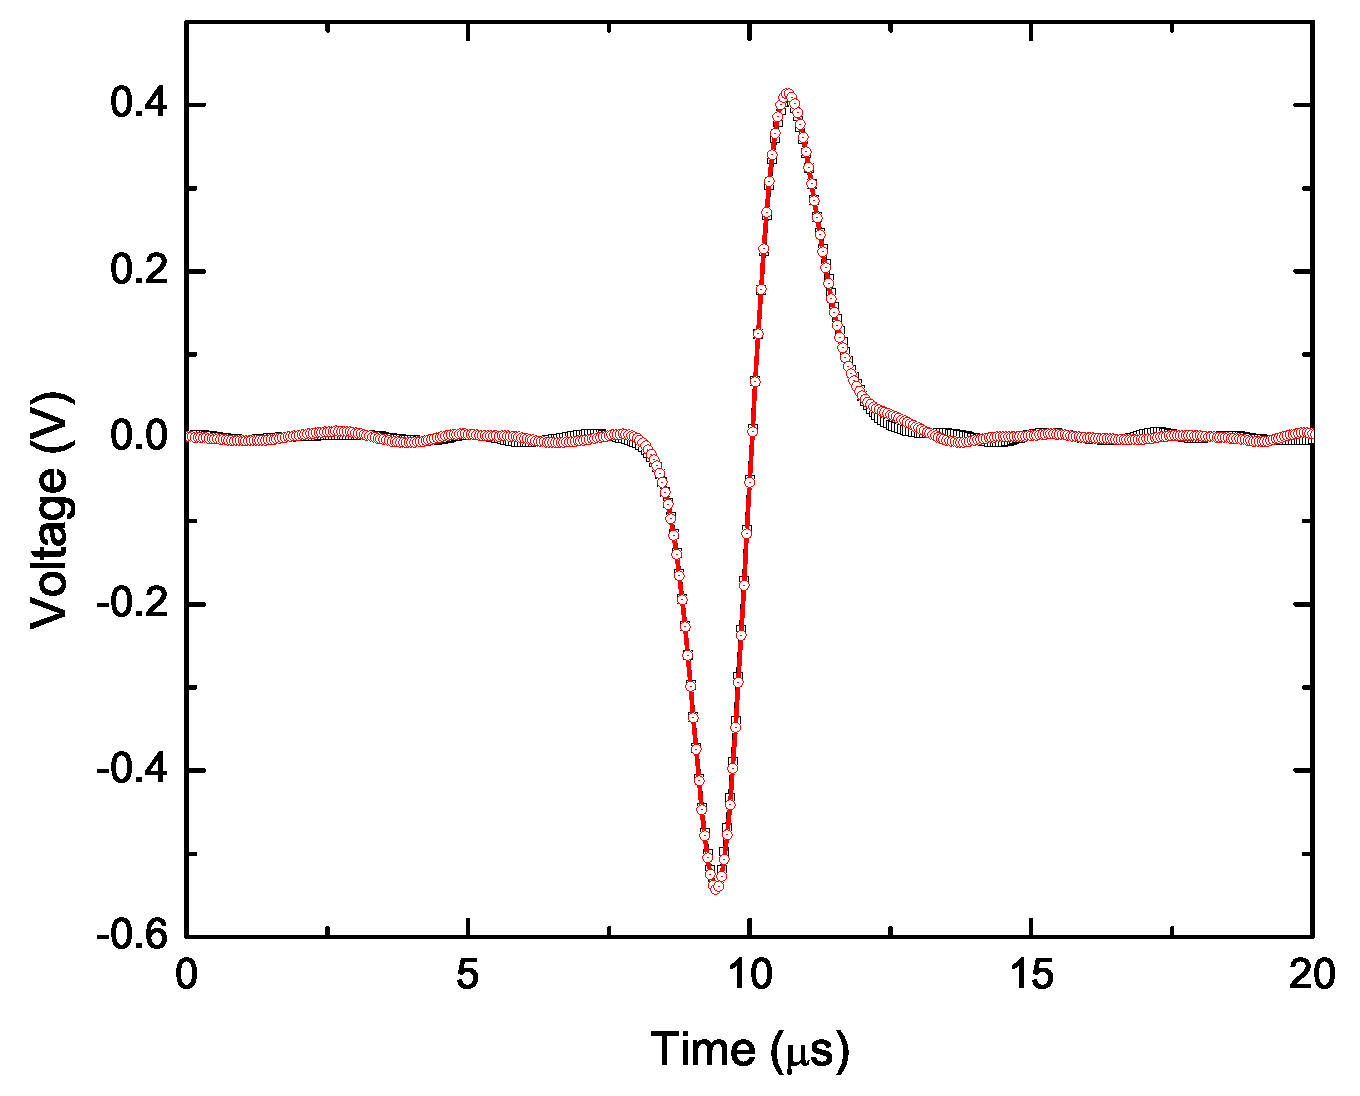
\includegraphics[width=0.6\linewidth]{pics/setup/AsFaradayCupBipolar}
	\caption{Bipolar output of the shaping amplifier. The peak-to-peak voltage is proportional to the total charge in the pulse. Two lines are plotted, both of which are the average of 1024 consecutive ion bunches. The peak-to-peak voltages agree, so the average charge has been determined quite accurately to be $1.17 \pm 0.02$~fC.\label{fig:AsFaradayCupBipolar}}
\end{figure}
Each line corresponds to the average over 1024 consecutive ion bunches. The experiment has been performed twice to get an idea of the reproducibility of the measurement. As it turns out, the two experiments agree very well, so that the charge for this experiment is determined to be $1.17 \pm 0.02$~fC.

The second step takes place within ten minutes of the charge determination: a voltage difference is applied over the MCP plates, so that it will act as a charge multiplier again. The applied voltage at the front of the MCP is $V_{in}=-1550$~V, while the rear of the MCP is at $V_{out}=0$~V. The phosphor screen is at a positive voltage of $V_{ph}=1000$~V. Now, the  output voltage of the transimpedance amplifier is averaged over 1024 consecutive ion bunches and this measurement is performed twice. The results are plotted in figure \ref{fig:AsMCPslowamp}. 
\begin{figure}[tbh!]
	\centering
		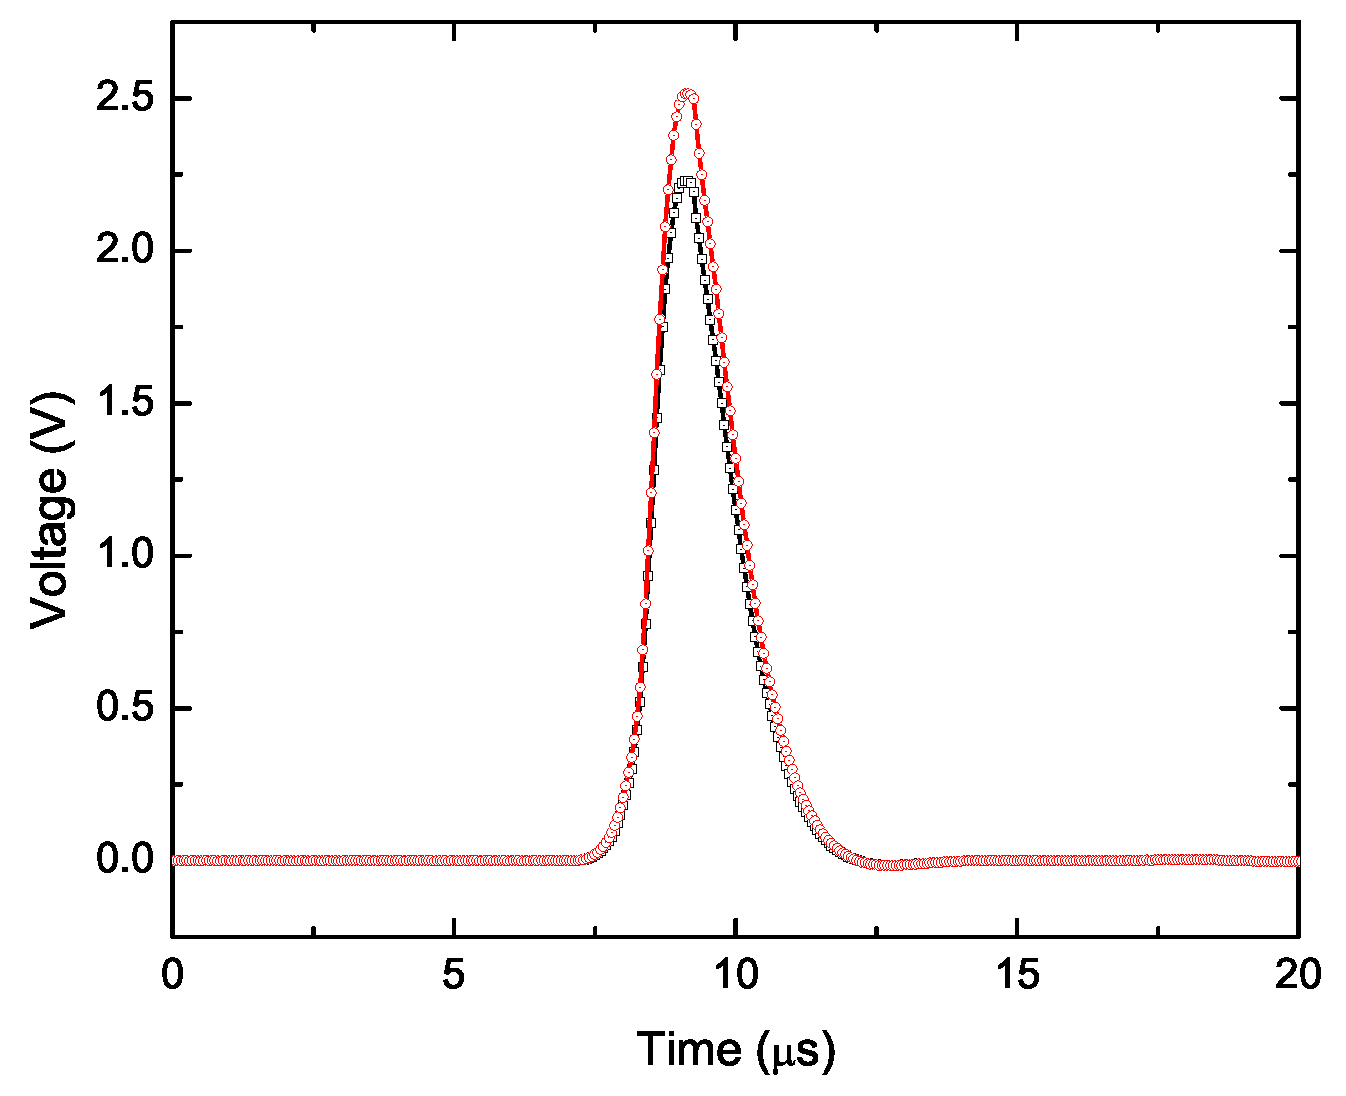
\includegraphics[width=0.6\linewidth]{pics/setup/AsMCPslowamp}
	\caption{The output of the trans-impedance amplifier, during the calibration measurement, where the different lines correspond to two identical series taken after each other. \label{fig:AsMCPslowamp}}
\end{figure}
In this case, there is some disagreement between the two measurements. This can be caused by a relatively small increase of the voltage over the MCP: a difference of only 7~V in terms of $\Delta_{MCP}=V_{out}-V_{in}$ could explain the change. This is in accordance with the voltage-stability of the high voltage supplies used to power the MCP. Hence, the minimal error margin of the current measurements is 10\%.
The signal needs to be integrated over time to get the charge of the bunch, which gives on average $(4.0 \pm 0.2)$~$\mu$V~s. This corresponds to a charge of $40 \pm 2$~pC (at a current to voltage conversion factor of 100 k$\Omega$) and hence a MCP gain of $(34 \pm 2) \times 10^3$.
The previous procedure can be repeated to relatively calibrate the MCP for other acceleration voltages and MCP potential differences.
%In figures \ref{fig:CalibrationMCP1550Accell6kV} and \ref{fig:CalibrationMCP1550Accell800V}, the voltage on the output of the trans-impedance amplifier is plotted versus the time.
%\begin{figure}[tbh!]
%    \subfloat[$V_a=6$~kV]{
%        \label{fig:CalibrationMCP1550Accell6kV}
%        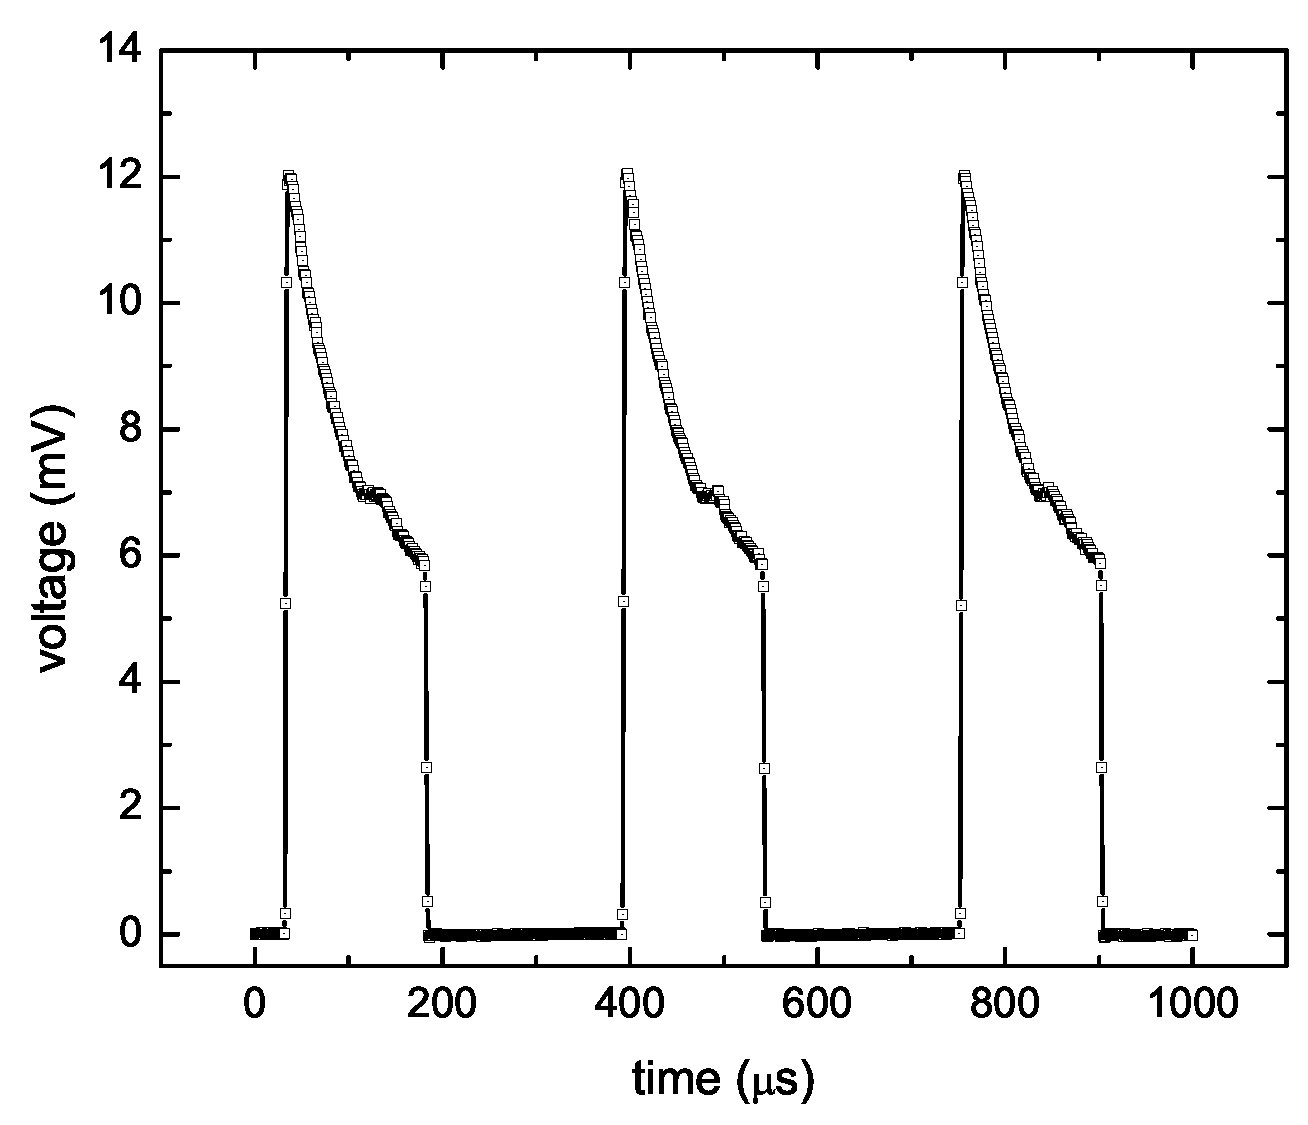
\includegraphics[width=0.48\linewidth]{CalibrationMCP1550Accell6kV}}
%    \hfill
%    \subfloat[$V_a=800$~V]{
%        \label{fig:CalibrationMCP1550Accell800V}
%        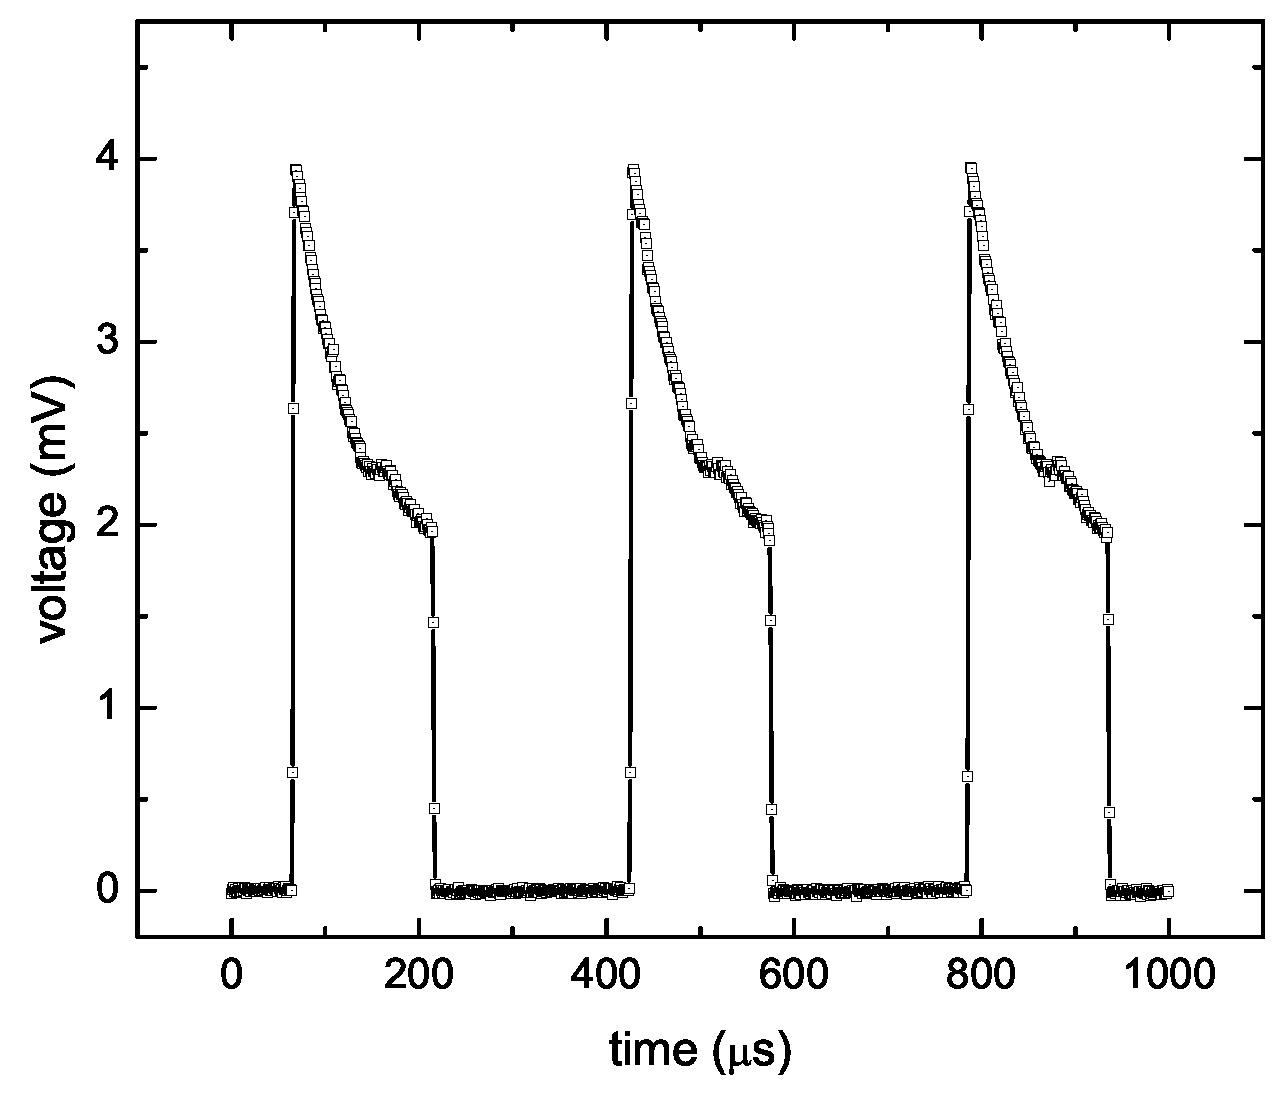
\includegraphics[width=0.48\linewidth]{CalibrationMCP1550Accell800V}}
%    \caption{Calibration experiment at an acceleration voltage of 6~kV and $\Delta_{MCP}=1550$~V, in panel (a). Panel (b) shows a calibration for an acceleration voltage of 800~V. The charge of the incoming ion bunches is determined by the integral of this signal.}
%    \label{fig:CalibrationMCP}
%\end{figure}
%In both figures, the plotted voltage is the average of 16384 ion bunches and they are performed with the same voltage over the MCP, namely $\Delta_{MCP}=1550$~V. The difference is the acceleration voltage, which is respectively 6~kV and 800~V. As can be seen, a lower acceleration voltage makes the time of flight for the ions longer, so that the measured current starts at a later time: the peak voltage is reached $32.5 \pm 0.5~\mu$s later. This is in good agreement with the expected value of $32.0~\mu$s, which can be obtained by assuming that the ions begin their acceleration exactly in the center of the MOT, accelerate for 1~cm to a kinetic energy corresponding to half the acceleration voltage, and travel at constant speed for 1.5~m. Another difference between the two figures is that the measured signal is weaker when a lower acceleration voltage is used. This can be explained by the quantum efficiency of the MCP, the probability that an electron is emitted when an ion hits the surface. If the ions arrive at higher energy, the quantum efficiency is typically higher, so on average more electrons will exit the MCP and hit the phosphor screen.
This is performed with $\Delta_{MCP}$ being 1500~V, 1600~V, 1650~V, 1700~V, 1750~V. The results of these experiments are plotted in figure \ref{fig:MCPcalibrationConstants}, which shows the gain of the MCP, plotted on a logarithmic scale, as a function of the voltage over the MCP, for an acceleration voltage $V_a=800$~V. 
As can be seen the gain increases almost exponentially with the voltage. This exponential relationship, which is a straight line in a logarithmic plot, has also been plotted as a dashed line in the figure. The linear relationship is obtained finding the solution of two equations with two unknowns (which are the two measurement points in the plot with the lowest voltage difference across the MCP plates). For higher voltages over the MCP a saturation effect occurs.
\begin{figure}[tbh!]
	\centering
		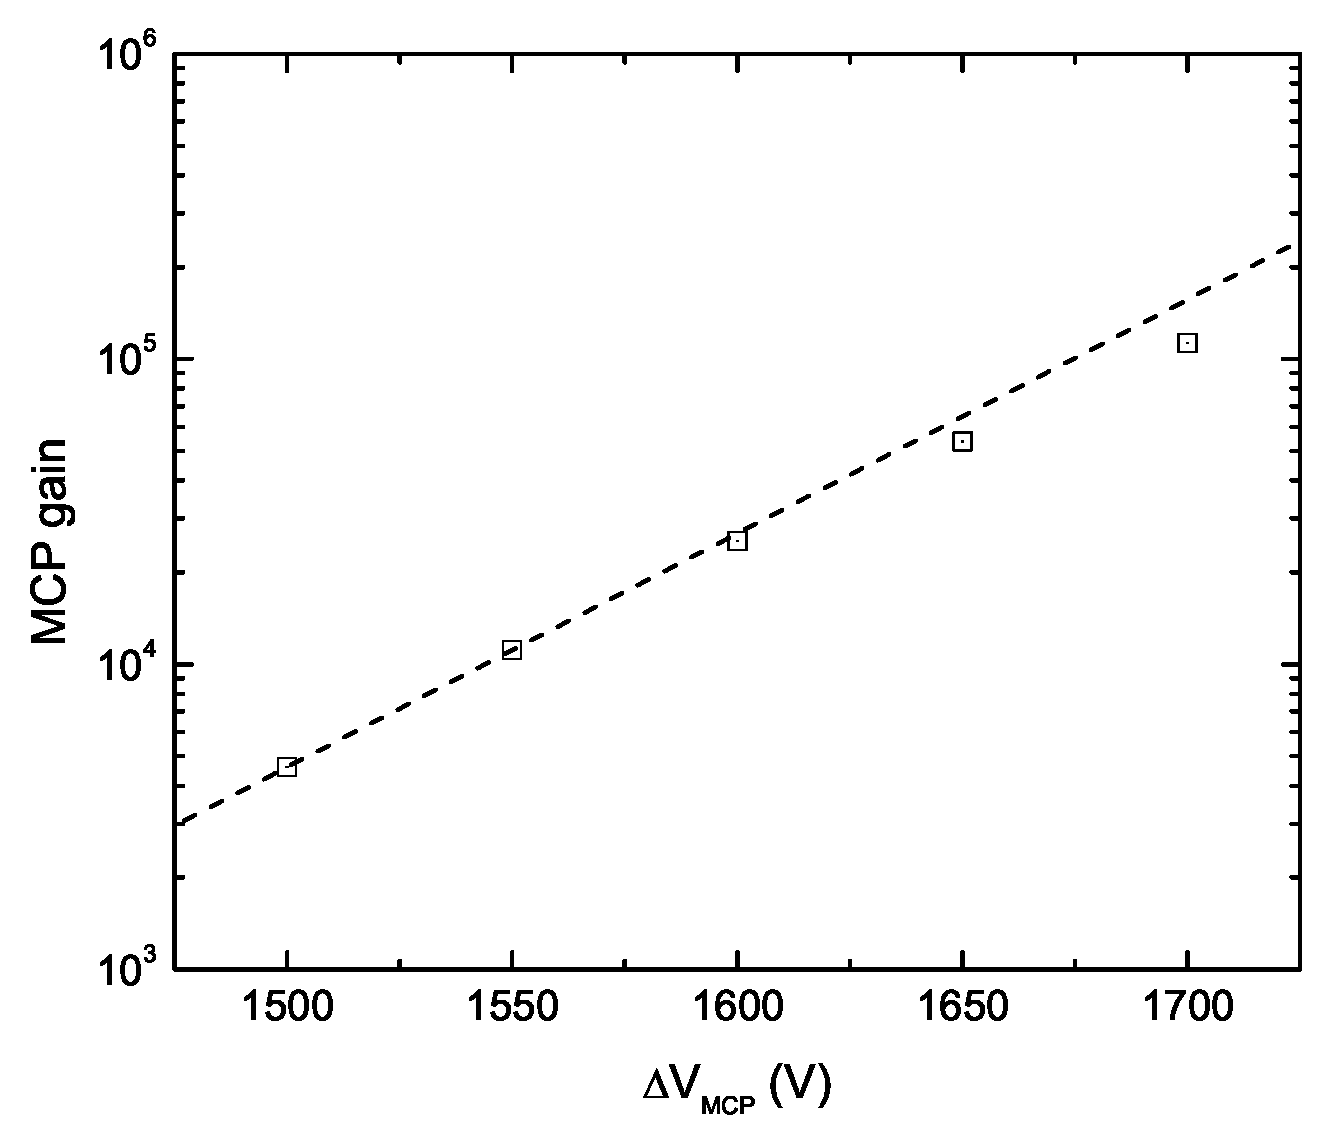
\includegraphics[width=0.6\linewidth]{pics/setup/MCPcalibrationConstants}
	\caption{The gain as determined by the calibration experiments for an acceleration energy $V_a=800$~V which correspond to a beam energy of about 400~eV. All points have a systematic error of about 10\%. The dashed line corresponds to an exponential increase of the gain, finding the solution through the first two points on the left hand side.\label{fig:MCPcalibrationConstants}}
\end{figure}

\section{Resolution of the detector \label{sec:resoMCP}}
The resolution of the detector has been determined experimentally by placing two pinholes, with diameters of 25~$\mu$m and 50~$\mu$m, downstream in front of the MCP. This is important for the measurement presented in chapter \ref{ch:tempmea}. Ion bunches with 3 keV energy are collimated by one of the two pinholes at a time. The \textit{rms}-radius $\sigma_a$ of an aperture with radius $r_p$ is given by
\begin{equation}
     \sigma_a = \sqrt{\frac{\int dx~x^2\sqrt{r_p^2-x^2}}{\int dx\sqrt{r_p^2-x^2}}}=\frac{r_p}{2}.
\end{equation}
The \textit{rms} spot radius $\sigma_{det}$ measured at the detector was substantially larger than $\sigma_a$, independently on the pinhole size used, as a result of the resolution of the detector. Figure \ref{fig:MCPresolution} shows one example obtained with the 25~$\mu$m pinhole, where a profile has been fitted with a Gaussian. 
\begin{figure}[tbh!]
	\centering
		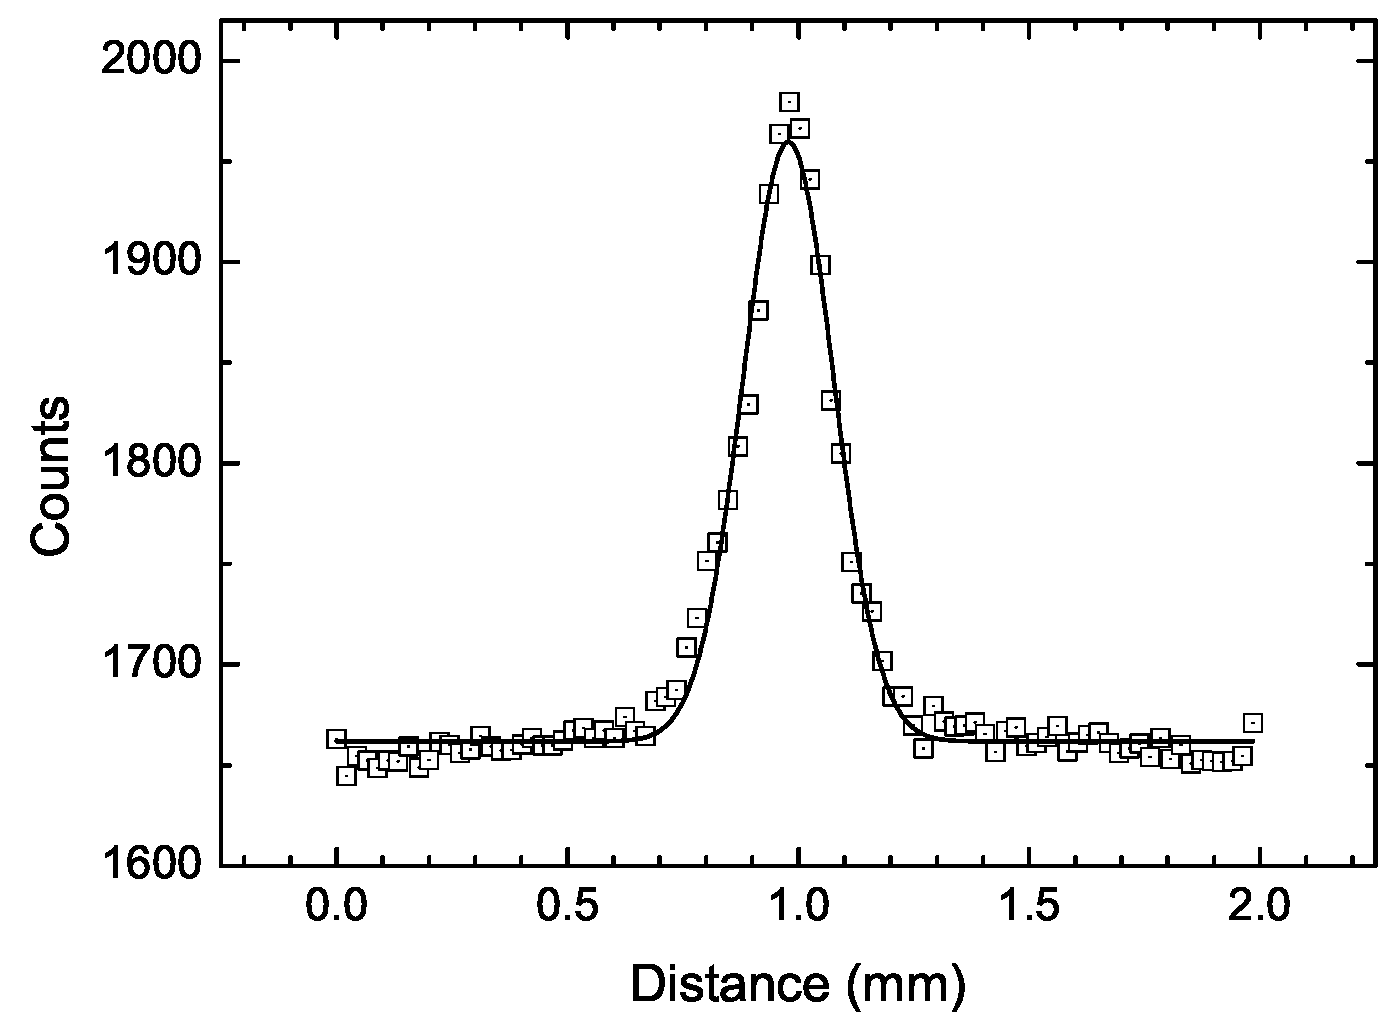
\includegraphics[width=0.7\linewidth]{pics/setup/MCPresolution}
	\caption{Plot profile of the spot size at the detector. The solid line is a Gaussian fit and it results in $\sigma_{det}=98~\mu$m.\label{fig:MCPresolution}}
\end{figure}
In this case, $\sigma_{det}=98~\mu$m. Multiple experiments, with both the pinholes, have been performed in order to obtain sufficient statistical accuracy. Using
\begin{equation}
     \sigma_{det} = \sqrt{\delta^2 + (1.2~\sigma_a)^2},
\end{equation}
the \textit{rms} resolution of the detector $\delta$ is found to be $(95 \pm 4)$ $\mu$m. Due to the expansion of the beam, the pinhole size at the position of the MCP has increased by 20\%.
\clearpage

\bibliographystyle{unsrt}

\begin{thebibliography}{10}

\bibitem{Reijnders2010}
M.~P. Reijnders.
\newblock {\em Ion beams from laser-cooled gases}.
\newblock PhD thesis, Eindhoven University of Technology, 2010.

\bibitem{Taban2009}
G~Taban.
\newblock {\em A cold atom electron source}.
\newblock PhD thesis, Eindhoven University of Technology, 2009.

\bibitem{Metcalf_Book_99}
H.J. Metcalf and P.~van~der Straten.
\newblock {\em {L}aser {C}ooling and {T}rapping}.
\newblock Springer, 1999.

\bibitem{Claessens06}
B.~J. Claessens.
\newblock {\em Dynamics and Applications of Excited Cold Atoms}.
\newblock PhD thesis, Eindhoven Technological University, 2006.

\bibitem{Hermans10}
K.H.M. Hermans.
\newblock {\em Measurement and modeling of Ultra Cold Ion current pulses}.
  {Bachelor's thesis, Eindhoven Technological University}, 2010.
  
\bibitem{vdHeijden11}
M.A. van~der Heijden.
\newblock {\em Creation and characterization of ultrashort ultracold electron
  bunches}.
\newblock Master's thesis, Eindhoven Technological University, 2011.
  
\end{thebibliography}

%\end{document}